\documentclass[11pt]{article}
\setlength{\oddsidemargin}{0in}
\setlength{\evensidemargin}{0in}
\setlength{\textwidth}{6.5in}
\setlength{\topmargin}{0in}
\setlength{\textheight}{8.5in}
\setlength{\headheight}{0pt}
\setlength{\headsep}{0pt}

\setcounter{topnumber}{3}%
\def\topfraction{.7}% 
\setcounter{bottomnumber}{1}
\def\bottomfraction{.3}
\setcounter{totalnumber}{5}%
\def\textfraction{.1}% was .2
\def\floatpagefraction{.7}% was .7
\setcounter{dbltopnumber}{2}
\def\dbltopfraction{.7}
\def\dblfloatpagefraction{.5}

\usepackage{clrscode3e}
\usepackage[parfill]{parskip}
\usepackage{textcomp}
\usepackage[T1]{fontenc}
\usepackage{titling}
\usepackage[shortlabels]{enumitem}
\usepackage[fleqn]{amsmath}
\usepackage{mathtools}
\usepackage{float}

% set title height
\setlength{\droptitle}{-4em}

% remove number from section
\makeatletter
\renewcommand{\@seccntformat}[1]{%
  \ifcsname prefix@#1\endcsname
    \csname prefix@#1\endcsname
  \else
    \csname the#1\endcsname\quad
  \fi}
\newcommand\prefix@section{}
\makeatother

% define how to make line breaks
\def\separateline{\medskip\hrule\medskip}

% for proofs
\usepackage{amsthm,amssymb}
\renewcommand{\qedsymbol}{\rule{0.7em}{0.7em}}

% get ceiling and floor functions
\DeclarePairedDelimiter{\ceil}{\lceil}{\rceil}
\DeclarePairedDelimiter\floor{\lfloor}{\rfloor}

% get degree symbol
\usepackage{gensymb}

% define title
\title{CS 31: Final Exam}
\author{Thomas Monfre}
\date{\today}

\begin{document}

\setlength{\abovedisplayskip}{0pt}

\maketitle

\section{Problem 1}
\separateline

\underline{\textbf{Part A:}} We are told a graph has a unique minimum spanning tree if, for every cut of the graph, there is a unique light edge crossing the cut. Since we are told the graph is connected, there exists at least one edge crossing each possible cut because all vertices are reachable from all other vertices. Then, since we are also told all edge weights are unique, there must exist a singular minimum-weight edge crossing each possible cut. Therefore, by the definition of a light edge, there must exist a unique light edge crossing each cut of the graph. Therefore, $G$ has a unique minimum spanning tree.

In order to show the second-best minimum spanning tree need not be unique, let us use the following counterexample.

\begin{figure}[ht]
    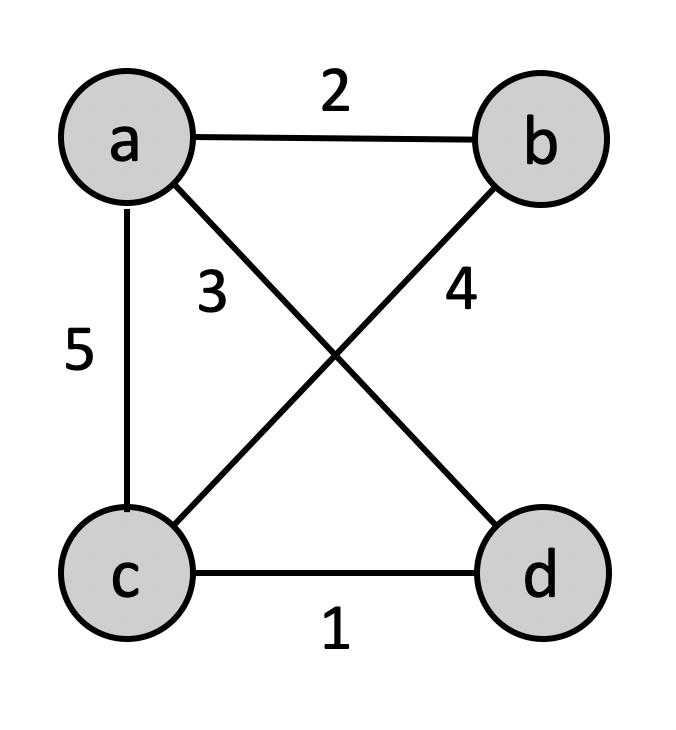
\includegraphics[width=1.5in]{prob1graph.png}
\end{figure}

For this example, let us first observe that each edge weight is a unique real-number. Then, the unique minimum spanning tree covers the edges $(c,d)$, $(d,a)$, $(a,b)$ for a total weight of 6. Then, there are two options for the second best minimum spanning tree. The first covers edges $(a,d)$ and $(b,c)$ for a total weight of 7, and the second covers edges $(d,c)$, $(c,b)$, and $(b,a)$ also yielding a total weight of 7. Therefore, the second best minimum spanning tree need not be unique.\\

\underline{\textbf{Part B:}} For this problem, let $T$ be a minimum spanning tree of $G$ and let $(u,v) \in T$ and $(x,y) \notin T$ be edges in $G$. Then, let us specify that $(x,y)$ is the minimum-weight edge among all edges in $G$ that are not in $T$. In order to prove $T - \{(u,v)\} \cup \{(x,y)\}$ is a second-best minimum spanning tree, let us construct a new spanning tree $T' = T - \{(u,v)\} \cup \{(x,y)\}$ by placing a specific restriction on $(u,v)$, then let us prove that $T'$ under this restriction is a second-best MST of $G$. To do so, let us initially set $T' = T$. In effect, we copy each edge from $T$ to $T'$.

Then, let us insert $(x,y)$ (the smallest weight edge not in $T$) into $T'$. Let us observe that doing so must create a cycle in $T'$. We know this to be the case because $T$ being a minimum spanning tree of $G$ indicates there exists a simple path between all vertices in $T$. Then, since we initially set $T' = T$, for some vertex $v \in T'$ there must exist a path in $T'$ from $v$ to $x$ and a path from $y$ to $v$, both of which do not traverse $(x,y)$ since $(x,y) \notin T$. Then, since $(x,y)$ was inserted into $T'$, there then must exist a cycle on $v$ since we can take the simple path $v \rightsquigarrow x$, then the edge $(x,y)$, then the simple path $y \rightsquigarrow v$ and arrive back at $v$.

Using this observation, since each edge weight is a distinct real-number, there must exist some edge $(u,v)$ of maximum weight on the cycle created in $T'$ that is not $(x,y)$. If we remove $(u,v)$ from $T'$, we then have that $T' = T - \{(u,v)\} \cup \{(x,y)\}$. Let us observe that $T'$ is now a spanning tree of $G$. We know this to be the case because $T'$ previously constructed a cycle on each vertex in the tree, and elementary graph theory states that removing a single edge from a cycle in an undirected graph will produce a path between all vertices on the cycle. Since all vertices in $T'$ (and therefore $G$) were on the cycle and the entire graph being cyclically connected indicates there cannot exist more than one cycle in $T'$ prior to removing $(u,v)$, upon removing $(u,v)$ from $T'$, there do not exist any cycles in $T'$, indicating there exists a simple path between all vertices in $T'$, thereby making $T'$ a spanning tree.

Using this, let us show that it must be the case that $w(x,y) > w(u,v)$. Since we defined $T$ to be an MST of $G$, $T$ and $T'$ differ by a single edge, and we proved above that $T'$ is a spanning tree of $G$, if $w(x,y) < w(u,v)$, then $T'$ would be a minimum spanning tree on $G$ and not $T$, contradicting our assumption that $T$ is a minimum spanning tree on $G$. Essentially, since we can reach all edges in each and the only difference between the two is a singular edge, the weight of the added edge in $T'$ must be greater than the removed edge in $T$, otherwise $T$ wouldn't have been an MST. Therefore, it must be the case that $w(x,y) > w(u,v)$. Note that we do not need to concern ourselves with equalities since all edge weights are distinct.

Then, it must be the case that $T'$ is a spanning tree on $G$ and $w(T) < w(T')$. Then, all that is left to prove is that $T'$ is a second best minimum spanning tree on $G$. To do so, let us prove that there does not exist a spanning tree on $G$ with a smaller total weight than $T'$ other than $T$. Observe that our choice of $(x,y)$ was the edge of smallest weight in $G$ that was not in $T$. Since the edge in $T$ that we removed from $T'$ was of maximum weight on the formed cycle, and the removed edge cannot be the added edge, the only way to minimize our increase in weight from $T$ to some new spanning tree we wish to form is to insert an edge of smaller weight than $(x,y)$ into that tree. We know this to be the case because we cannot remove an edge of larger weight originally in $T$ than $(u,v)$ without contradicting our choice of $(u,v)$. Then, since all edge weights are distinct and we defined $(x,y)$ as the edge of smallest weight not in $T$, we cannot insert an edge not in $T$ into our new tree other than $(x,y)$ without contradicting our choice of $(x,y)$. We know this to be the case because there cannot exist an edge not in $T$ of smaller weight than $(x,y)$. Therefore, there cannot exist a spanning tree on $G$ of smaller total weight than $T'$ other than $T$ since no edges that are not in $T$ exist with a smaller weight than $(x,y)$ that we could swap out to produce a smaller total weight.

Therefore, since $T'$ is a spanning tree on $G$, $w(T) < w(T')$, and there does not exist a spanning tree $T''$ on $G$ such that $w(T) < w(T'') < w(T')$, $T'$ must be a second-best minimum spanning tree on $G$. Then, since $T' = T - \{(u,v)\} \cup \{(x,y)\}$, we have the claim.\\

\underline{\textbf{Part C:}} In order to compute the maximum edge weight of all edges on a path between two vertices $u$ and $v$ in a minimum spanning tree $T$, let us pursue a dynamic programming solution. To do so, let us take advantage of the inherently optimal substructure that exists in all paths of a minimum spanning tree. Since there exists one and only one path between some vertices $v_1$ and $v_k$ in $T$, the maximum weight edge on the path is either the largest weight edge on the path $v_1 \rightsquigarrow v_{k-1}$ or the edge weight $w(v_{k-1},v_k)$. Then, we can build the matrix $max$ in a bottom-up fashion and use the previously computed solution for the path $v_1 \rightsquigarrow v_{k-1}$ as well as the edge weight $w(v_{k-1},v_k)$ in order to correctly compute $max[v_1,v_k]$. Let us note, however that since $max[v_1,v_k]$ stores the identity of an edge and not its weight, we must construct a helper matrix $weights$ in which $weights[v_1,v_k]$ stores the weight of the edge referenced at $max[v_1,v_k]$.

Using this, we then simply must search the minimum spanning tree (which by definition reaches all edges in $G$), and set our maximum edge weight estimation using the above optimal substructure. Let us note, however, that searching the tree depends on where our search originates from. Depending on the source of each search, we may arrive at different results for the maximum weight edge on each path since some source vertices may only lie on just part of the entire path. Therefore, we must run a search from each possible start vertex and store the optimal solution among all start vertices.

Then, in order to search the minimum spanning tree, let us simply run \proc{Breadth-First-Search} from each vertex in the tree. We will only consider edges in $G$ that are in $T$. Each time we iterate over a vertex $v$ in a vertex $u$'s adjacency list, we have an edge $(u,v)$ in $T$. Then, there must exist a path $s \rightsquigarrow u$ in $T$ and we must have previously iterated over the edges on that path in order to be observing the edge $(u,v)$. Then, our optimal substructure, as defined above, takes hold. Specifically, our largest edge weight estimate for the path $s \rightsquigarrow v$ is either the maximum edge weight on the path $s \rightsquigarrow u$ or $w(u,v)$ depending on which is larger. Since the matrix $max[s,u]$ stores the identity of the maximum weight edge on the path $s \rightsquigarrow u$ and $weights[s,u]$ holds the weight of that edge, we simply must check if $w(u,v) > weights[s,u]$. If so, we set $max[s,v] = (u,v)$ and $weights[s,v] = w(u,v)$. Otherwise, we set $max[s,v] = max[s,u]$ and $weights[s,v] = weights[s,u]$. Note that we will initialize the $weights$ matrix such that each value is $-\infty$.

Then, after a single run of this modified \proc{BFS}, we will have computed a largest weight estimate for each possible path. Let us note that since \proc{BFS} runs in $O(V+E)$ time and $|E| \leq |V| - 1$ in a minimum spanning tree, we then have $O(V)$ for a single call to \proc{BFS}. Since we call \proc{BFS} from each possible source vertex, of which there are $|V|$, we then have a total run-time of $O(V^2)$ for this algorithm.

We can prove the correctness of this algorithm by observing that our optimal substructure, as outlined above, holds for all possible source vertices. We know this to be the case because \proc{BFS} visits vertices in order from the source. Therefore, every time we come across an edge $(u,v)$ in \proc{BFS}, we must have previously discovered a path from $s$ to $u$ and therefore must have computed some solution for the maximum edge weight on the path. Furthermore, since we initialize each value in the $weights$ matrix to be $-\infty$, the first time we discover a particular path, we will set the maximum edge weight estimate on that path to be the weight of the currently observed edge.

Therefore, given a minimum spanning tree $T$, we can correctly compute $max[u,v]$ for all $u,v \in V$ in $O(V^2)$ time.\\

\underline{\textbf{Part D:}} In order to compute the second-best minimum spanning tree of $G$, let us bring everything we have proven thus far together. To do so, we will first compute the minimum spanning tree $T$ of $G$. To do so, let us use \proc{MST-Prim} which runs in time $O(E + V\lg{V})$ using a priority queue implemented with a Fibonacci heap. Then, we will create a new tree $T'$ that we will eventually compute to be the second-best minimum spanning tree of $G$. Let us initialize $T'$ to $T$ in time $O(V + E)$ since we must copy each vertex and each edge.

Then, let us construct the $max$ matrix from $T$ using the algorithm described in part c of this problem. This gives us a matrix of references to edges of maximum weight in $T$ on a path between all pairs of vertices. Then, we seek to find the smallest weight edge of all edges not in $T$. In order to determine this, let us iterate over all $|E|$ edges in $G$. For some edge $(u,v) \in G.E$, if $(u,v) \notin T$, then we check its weight. If $w(u,v)$ is less than the smallest weight we've found so far, we update our reference to the minimum edge weight not in $T$. Then, after iterating over all $|E|$ edges, we will have a reference to the edge of smallest weight not in $T$. Let us note that this takes time $O(E)$ to complete, but since $|E| \leq |V|*(|V|-1)$, we can bound $O(E) = O(V^2)$.

Then, we have the smallest weight edge in $G$ that is not in the minimum spanning tree $T$. Let us refer to this edge as $(x,y)$. Then, let us insert $(x,y)$ into $T'$. Note that this forms a cycle in $T'$, as per our proof in part b of this problem. Then, following our proof from part b, we seek to remove the edge of largest weight on the cycle that is formed that was originally in $T$. Note that at this point $T' = T \cup (x,y)$ since we made a copy of $T$ then inserted $(x,y)$ into it. Therefore, let us use the $max$ matrix computed above. This matrix holds a reference to the edge of largest weight on a path between all pairs of vertices in $T$. Since by the definition of a minimum spanning tree, all vertices must be reachable in $T$, there then must exist a path in $T$ from $y$ to $x$. We know this to be the case because adding $(x,y)$ to $T'$ created a cycle.

Therefore, the edge of largest weight on the cycle formed by inserting $(x,y)$ into $T'$ that was originally in $T$ is the edge of largest weight on the path from $y$ to $x$ in $T$. Then, we can make a constant time look-up to $max[y,x]$ to retrieve a reference to this edge. Let us refer to this edge as $(u,v)$. With this reference, let us then remove $(u,v)$ from $T'$. Note that, per our proof to part b of this problem, this removes the cycle formed in $T'$ from inserting $(x,y)$. Then, $T' = T - \{(u,v)\} \cup \{(x,y)\}$. As per our proof from part b, $T'$ is therefore a second-best minimum spanning tree of $G$.

Then, the run-time of this algorithm is: $O(E + V\lg{V})$ for the call to \proc{MST-Prim}. $O(V+E)$ for setting $T' = T$. $O(V^2)$ for computing the $max$ matrix. $O(E)$ for finding the minimum weight edge not in $T$. $O(1)$ for inserting $(x,y)$ into $T'$ and $O(1)$ for computing $max[y,x]$ and removing it from $T'$. Then, since there exist at most $|V|*(|V|-1)$ edges in $G$ and we know $|V| > |E|$ for $T$ since $T$ is a minimum spanning tree, we can bound the sum of all of these operations by $O(V^2)$. Therefore, we have a final run-time of $O(V^2)$ for computing the second-best minimum spanning tree of $G$.

\newpage

\section{Problem 2}
\separateline

\underline{\textbf{Part A:}} If $\delta(s,v) \leq |E|$ for all vertices $v \in V$, then in order to show how to compute $\delta(s,v)$ for all $v \in V$ in $O(E)$ time, let us take advantage of our bound on shortest path weights. To do so, let us make a call to \proc{Dijkstra} and use the given bound on shortest path weights to implement a more efficient priority queue. Specifically, let us implement this priority queue with a direct addressing array of size $|E| + 2$ where each index $i=0...|E| + 1$ in the array holds a doubly linked list with sentinel of vertices such that each vertex $v$ in the linked list at index $i$ has a shortest path estimate $v.d = i$. The only exception to this is if $v.d = \infty$ (which is the initialized condition from \proc{Initialize-Single-Source}). In such a case, we will hold $v$ in index $|E| + 1$ since we know that no shortest path estimate may be greater than $|E|$ and we therefore will never put a vertex with a shortest path estimate of $\infty$ and another vertex with a shortest path estimate of $|E| + 1$ in the same linked list.

Then, we can implement \proc{Insert} for a given vertex $v$ in constant time by performing a constant-time lookup into the addressing array for the linked list at index $v.d$, then inserting the vertex at the end of the doubly linked list with sentinel. If $v.d = \infty$, we will insert $v$ into the linked list at index $|E| + 1$. We can implement \proc{Decrease-Key} in constant time given a reference to a vertex in a linked list by updating its shortest distance estimate, removing it from its current linked list in constant time, then inserting it back into the direct addressing array with a constant time call to \proc{Insert}.

Lastly, we can implement \proc{Extract-Min} in $O(E)$ time across all $|V|$ calls to \proc{Extract-Min} by holding a reference to the index in the direct addressing array that holds a minimum value in the queue. Let us refer to this reference as $minIndex$. We will initialize $minIndex$ to 0. For each call to \proc{Extract-Min}, we will first check if the linked list at index $minIndex$ is empty. If it is, then we increment $minIndex$ by 1 and check again. If it is not, then we simply remove the first vertex in the linked list at index $minIndex$ and return it. Then, the only thing left to prove is that there will never exist a vertex in the table in a linked list at an index less than $minIndex$. We know this to be the case because we insert all vertices into the priority queue in \proc{Dijkstra} before ever making a call to \proc{Extract-Min}, so we can never insert new vertices into the queue after a call to \proc{Extract-Min}. Furthermore, since we are told that all edge weights are non-negative, upon setting $v.d = u.d + w(u,v)$ in the \proc{Relax} method, it must be that $w(u,v) \geq 0$ and $u.d \geq 0$ so $v.d \geq u.d$. Then, since the vertex $u$ is the vertex that was most recently extracted from the queue and the value that we decreased $v.d$ to must be greater than or equal to $u.d$, it cannot be that we will ever set a shortest path estimate (key) in the queue to something less than $minIndex$. Therefore, since we iterate through the direct addressing array exactly once and make constant time look-ups along the way, we can implement all $|V|$ calls to \proc{Extract-Min} in $O(E)$ time.

Therefore, implementing \proc{Dijkstra} with this priority queue yields $O(V)$ for all $|V|$ calls to \proc{Insert}, $O(E)$ for all $|E|$ calls to \proc{Decrease-Key}, and $O(E)$ for all $|V|$ calls to \proc{Extract-Min}. Therefore, the run-time of \proc{Dijkstra} in this case will be $O(V+E)$. Since, we are told $|E| \geq |V| - 1$, however, we can simplify this to $O(E)$. We can prove the correctness of this algorithm with \textbf{Theorem 24.6} from CLRS Chapter 24.3 which proves \proc{Dijkstra} computes the shortest path weight from a source vertex to all vertices in a graph, thereby computing $\delta(s,v)$ for all $v \in V$ in $O(E)$ time.\\

\underline{\textbf{Part B:}} Since $\delta_1(s,v)$ is defined as the shortest path weight from the source vertex $s$ to some vertex $v$ using weight function $w_1$, and $w_1(s,v)$ is the scaled down version of $w(s,v)$ given by the single most significant bit of $w(s,v)$, and each bit is either a 0 or a 1, we know that each edge in $G$ defined by $w_1$ has a weight of 0 or 1. Therefore, in the worst case, the shortest path from $s$ to $v$ traverses every edge in $G$ and each edge weight is 1. In such a case, the worst case and therefore greatest possible shortest path weight in the graph would be $|E|$. Therefore, we can conclude that $\delta_1(s,v) \leq |E|$ for all $v \in V$. Then, we have the conditions described in part A of this problem, and therefore can use the solution outlined and proved above in order to compute $\delta_1(s,v)$ for all $v \in V$ in $O(E)$ time.\\

\underline{\textbf{Part C:}} First let us prove that for $i=2,3,...k$ we have either $w_i(u,v) = 2w_{i-1}(u,v)$ or $w_i(u,v) = 2w_{i-1}(u,v) + 1$. We are told $w_i(u,v) = \floor{\frac{w(u,v)}{2^{k-i}}}$ in the problem description. Then, $w_{i-1}(u,v) = \floor{\frac{w(u,v)}{2^{k-(i-1)}}}$, so $2w_{i-1}(u,v) = 2\floor{\frac{w(u,v)}{2^{k-(i-1)}}}$.

By the nature of mathematical floors, $\floor{x} \leq x < \floor{x} + 1$ for some $x$ therefore $2\floor{x} \leq 2x < 2\floor{x} + 2$. Then, since equation 3.7 in CLRS Chapter 3.2 states $\floor{\frac{a}{b}} \geq \frac{a - (b-1)}{b}$, we have that $\floor{2x} - 1 \geq 2x$  if we set $a=x$ and $b=1/2$ and simplify. Then, since we have $2\floor{x} \leq 2x < 2\floor{x} + 2$ and $2x \leq \floor{2x} - 1$, we have $2\floor{x} \leq 2x \leq \floor{2x} - 1 < 2\floor{x} + 2$. We then also have that $\floor{2x} - 1 < 2\floor{x} + 1 \leq \floor{2x} < 2\floor{x} + 2$. Therefore, it must be that $2\floor{x} = \floor{2x} - 1$ or $2\floor{x} = \floor{2x}$ for some arbitrary $x$ by the inequalities listed above.

Substituting $\floor{\frac{w(u,v)}{2^{k-(i-1)}}}$ for $x$, we then have $2w_{i-1}(u,v) = 2  \floor{\frac{w(u,v)}{2^{k-(i-1)}}} = \floor{\frac{2w(u,v)}{2^{k-(i-1)}}}$, or $2w_{i-1}(u,v) = 2  \floor{\frac{w(u,v)}{2^{k-(i-1)}}} = \floor{\frac{2w(u,v)}{2^{k-(i-1)}}} - 1$. Then, observe that $\floor{\frac{2w(u,v)}{2^{k-(i-1)}}} = \floor{\frac{w(u,v)}{2^{k-i}}} = w_i(u,v)$.

Then, we have that $2w_{i-1}(u,v) = w_i(u,v)$ or $2w_{i-1}(u,v) = w_i(u,v) - 1$. Therefore, for $i=2,3,...k$ we have either $w_i(u,v) = 2w_{i-1}(u,v)$ or $w_i(u,v) = 2w_{i-1}(u,v) + 1$. Hence, the claim.

Let us note that this makes sense in the context of the problem. By the definition of bits, when we shift all bits one position to the left and insert a bit at the far right, the value of each bit in the original number will double. A 1 in the least most significant position will become worth 2. A 1 in the position to the left of that will become worth 4, and so on. Therefore, when we insert a bit at the far right, any 1 in a bit position will now be worth twice of what it was previously. Then, since the inserted bit to the far right is worth either 0 or 1, and $w_{i}$ contains one more bit at the far right than $w_{i-1}$, it must be the case that $w_i(u,v) = 2w_{i-1}(u,v)$ or $w_i(u,v) = 2w_{i-1}(u,v) + 1$, depending on the value of the inserted bit at the far right.\\

Using this, let us then prove $2\delta_{i-1}(s,v) \leq \delta_i(s,v) \leq 2\delta_{i-1}(s,v) + |V| - 1$ for all $v \in V$. To do so, let us consider the worst case in which the shortest path from $s$ to $v$ traverses all vertices in $G$. Let us define this shortest path $p = \langle s, v_1, v_2, ..., v_{|V| - 1} \rangle$. Note that $v_{|V|-1} = v$ and that we refer to this vertex as $v_{|V| - 1}$ because we are considering the case in which the path traverses all vertices and we put the source vertex in the path. Therefore, $p$ contains a total of $|V| - 1 + 1 = |V|$ vertices.

Then, by the definition of $\delta$ in the problem definition, $\delta_i(s,v) = w_i(s,v_1) + \sum\limits_{j=1}^{|V| - 2}{w_i(v_j, v_{j+1})}$. Note that we iterate from $j=1$ to $|V| - 2$ because we handle the source vertex in $w_i(s,v_1)$ and since we access $v_{j+1}$ in the summation, the last vertex we should iterate on is $v_{|V| - 2}$ so we access the last edge $(v_{|V|-2}, v_{|V|-1})$ within the summation.

By the inequality proven above, we know $w_i(u,v) = 2w_{i-1}(u,v)$ or $w_i(u,v) = 2w_{i-1}(u,v) + 1$. Let us first consider the case in which $w_i(u,v) = 2w_{i-1}(u,v)$ for all $(u,v)$ on the shortest path $p$. In this case, we have the following:

\hspace*{3mm}
\begin{equation}
\begin{split}
\delta_i(s,v) &= w_i(s,v_1) + \sum\limits_{j=1}^{|V| - 2}{w_i(v_j, v_{j+1})}\\
              &= 2w_{i-1}(s,v_1) + \sum\limits_{j=1}^{|V| - 2}{2w_{i-1}(v_j, v_{j+1})}\\
              &= 2w_{i-1}(s,v_1) + 2\sum\limits_{j=1}^{|V| - 2}{w_{i-1}(v_j, v_{j+1})}\\
              &= 2\Big(w_{i-1}(s,v_1) + \sum\limits_{j=1}^{|V| - 2}{w_{i-1}(v_j, v_{j+1})} \Big)\\
              &= 2\delta_{i-1}(s,v) $~~ by the definition of $\delta
\end{split}
\end{equation}

Let us now consider the case in which $w_i(u,v) = 2w_{i-1}(u,v) + 1$ for all $(u,v)$ on the shortest path $p$. In this case, we have the following:

\hspace*{3mm}
\begin{equation}
\begin{split}
\delta_i(s,v) &= w_i(s,v_1) + \sum\limits_{j=1}^{|V| - 2}{w_i(v_j, v_{j+1})}\\
              &= 2w_{i-1}(s,v_1) + 1 + \sum\limits_{j=1}^{|V| - 2}{2w_{i-1}(v_j, v_{j+1}) + 1}\\
              &= 2w_{i-1}(s,v_1) + 1 + |V| - 2 + \sum\limits_{j=1}^{|V| - 2}{2w_{i-1}(v_j, v_{j+1})}\\
              &= 2w_{i-1}(s,v_1) + |V| - 1 + 2\sum\limits_{j=1}^{|V| - 2}{w_{i-1}(v_j, v_{j+1})}\\
              &= 2 \Big(w_{i-1}(s,v_1) + \sum\limits_{j=1}^{|V| - 2}{w_{i-1}(v_j, v_{j+1})} \Big) + |V| - 1\\
              &= 2\delta_{i-1}(s,v) + |V| - 1  $~~ by the definition of $\delta
\end{split}
\end{equation}

Then, we know if $w_i(u,v) = 2w_{i-1}(u,v)$ for all $(u,v)$ we have $\delta_i(s,v) = 2\delta_{i-1}(s,v)$ and if $w_i(u,v) = 2w_{i-1}(u,v) + 1$ for all $(u,v)$ we have $\delta_i(s,v) = 2\delta_{i-1}(s,v) + |V| - 1$. Then for some $(u,v)$ on the path, since $w_i(u,v)$ could equal $2w_{i-1}(u,v)$ or $2w_{i-1}(u,v) + 1$, we then have $2\delta_{i-1}(s,v) \leq \delta_i(s,v) \leq 2\delta_{i-1}(s,v) + |V| - 1$. Essentially, the case in which $\delta_i(s,v) = 2\delta_{i-1}(s,v)$ is a worst case in which all edge weights are $2w_{i-1}(u,v)$ and the case in which $\delta_i(s,v) = 2\delta_{i-1}(s,v) + |V| - 1$ is a worst case in which all edge weights are $2w_{i-1}(u,v) + 1$. Since each edge weight in reality could be either, we can then bound $\delta_i(s,v)$ by $2\delta_{i-1}(s,v) \leq \delta_i(s,v) \leq 2\delta_{i-1}(s,v) + |V| - 1$. Since we observed the worst case in which the shortest path traverses every vertex, we have the claim.\\

\underline{\textbf{Part D:}} Next, let us prove $\hat{w_i}(u,v) = w_i(u,v) + 2\delta_{i-1}(s,u) - 2\delta_{i-1}(s,v)$ is a non-negative integer for all $i=2,3,...k$ and all $u,v \in V$. First, let us observe that we proved above that $w_i(u,v) = 2w_{i-1}(u,v)$ or $w_i(u,v) = 2w_{i-1}(u,v) + 1$ for all $i=2,3,...k$ and all $u,v \in V$. Note that both of these values are non-negative integers because the problem description states every edge weight for all $i$ is a non-negative integer. Then, since we seek to prove $\hat{w_i}(u,v)$ is a non-negative integer, the worst-case is that in which $w_i(u,v) = 2w_{i-1}(u,v)$ since $2w_{i-1}(u,v) < 2w_{i-1}(u,v) + 1$ and we add $w_i(u,v)$ to $\hat{w_i}(u,v)$.

Then, we can re-write the above equation to $\hat{w_i}(u,v) = 2w_{i-1}(u,v) + 2\delta_{i-1}(s,u) - 2\delta_{i-1}(s,v) = 2\Big( w_{i-1}(u,v) + \delta_{i-1}(s,u) - \delta_{i-1}(s,v) \Big)$. Note that $w_{i-1}(u,v) \geq 0$ by the problem definition. Then, let us observe that $\delta_{i-1}(s,u)$ is the total weight of the shortest path $s \rightsquigarrow u$ in $G$, and $\delta_{i-1}(s,v)$ is the total weight of the shortest path $s \rightsquigarrow v$ in $G$.

Then, there exists two cases: the shortest path $s \rightsquigarrow v = s \rightsquigarrow u + (u,v)$ or it does not -- i.e. the shortest path from $s$ to $v$ traverses the shortest path from $s$ to $u$ plus the edge $(u,v)$ or it does not. If $s \rightsquigarrow v = s \rightsquigarrow u + (u,v)$, then $w_{i-1}(u,v) + \delta_{i-1}(s,u) = \delta_{i-1}(s,v)$. Then, $\hat{w_i}(u,v) = 2\Big( w_{i-1}(u,v) + \delta_{i-1}(s,u) - \delta_{i-1}(s,v) \Big) = 0$ and since 0 is a non-negative integer, we have the claim.

If $s \rightsquigarrow v \neq s \rightsquigarrow u + (u,v)$, then we have two cases. Either $s \rightsquigarrow v$ traverses $s \rightsquigarrow u$ or it does not. If $s \rightsquigarrow v$ traverses $s \rightsquigarrow u$, then since $s \rightsquigarrow v \neq s \rightsquigarrow u + (u,v)$, it must take some path $u \rightsquigarrow v$ that is not the edge $(u,v)$. In this case, $u \rightsquigarrow v$ must have a smaller total edge weight than $(u,v)$ since $s \rightsquigarrow v$ is a shortest weight path. Then, $s \rightsquigarrow v = s \rightsquigarrow u + u \rightsquigarrow v$ and $\delta_{i-1}(u,v) < w_{i-1}(u,v)$, so we have $\hat{w_i}(u,v) = 2\Big( w_{i-1}(u,v) + \delta_{i-1}(s,u) - \delta_{i-1}(s,u) - \delta_{i-1}(u,v) \Big) = 2\Big( w_{i-1}(u,v) - \delta_{i-1}(u,v) \Big) \geq 0.$

If $s \rightsquigarrow v$ does not traverse $s \rightsquigarrow u$, then $s \rightsquigarrow v$ cannot traverse $(u,v)$ since if it did, there must be a path of smaller weight from $s$ to $u$ in $G$, contradicting the assumption that $s \rightsquigarrow u$ is the smallest weight path from $s$ to $u$. Therefore, $s \rightsquigarrow v$ does not overlap with $s \rightsquigarrow u$ or $(u,v)$. Then, since $s \rightsquigarrow v$ is the smallest weight path from $s$ to $v$ and it does not traverse $s \rightsquigarrow u$ or $(u,v)$, it must be that $\delta_{i-1}(s,v) \leq \delta_{i-1}(s,u) + w_{i-1}(u,v)$. Then, $\hat{w_i}(u,v) = 2\Big( w_{i-1}(u,v) + \delta_{i-1}(s,u) - \delta_{i-1}(s,v) \Big) \geq 0$.

Then, since we have shown $\hat{w_i}(u,v) \geq 0$ for all possible cases, $\hat{w_i}(u,v)$ is a non-negative integer. Hence, the claim.\\

\underline{\textbf{Part E:}} In order to prove $\delta_i(s,v) = \hat{\delta_i}(s,v) + 2\delta_{i-1}(s,v)$ let us again take the worst case scenario in which the smallest weight path from $s$ to $v$ traverses each vertex in $G$. We will then use our definition above of this path $p = \langle s, v_1, v_2, ..., v_{|V| - 1} \rangle$, where $v_{|V|-1} = v$. Then, by our definition from above $\delta_i(s,v) = w_i(s,v_1) + \sum\limits_{j=1}^{|V| - 2}{w_i(v_j, v_{j+1})}$. We will then use this to show $\hat{\delta_i}(s,v) = w_i(s,v_1) + \sum\limits_{j=1}^{|V| - 2}{w_i(v_j, v_{j+1})} - 2\delta_{i-1}(s,v) = \delta_i(s,v) - 2\delta_{i-1}(s,v)$. Doing so will then prove that $\delta_i(s,v) = \hat{\delta_i}(s,v) + 2\delta_{i-1}(s,v)$.\\

To start, let us break down $\hat{\delta_i}(s,v)$ into its requisite parts. Using the formula above, we have $\hat{\delta_i}(s,v) = \hat{w_i}(s,v_1) + \sum\limits_{j=1}^{|V| - 2}{\hat{w_i}(v_j, v_{j+1})}$. Then, using the equation for $\hat{w_i}$ proven above, we have $\hat{w_i}(s,v_1) = w_i(s,v_1) + 2\delta_{i-1}(s,s) - 2\delta_{i-1}(s,v_1)$. Note that $2\delta_{i-1}(s,s) = 0$ so $\hat{w_i}(s,v_1) = w_i(s,v_1) - 2\delta_{i-1}(s,v_1)$.

Then, in order to break down $\sum\limits_{j=1}^{|V| - 2}{\hat{w_i}(v_j, v_{j+1})}$, let us observe that $\hat{w_i}(v_j, v_{j+1}) = w_i(v_j,v_{j+1}) + 2\delta_{i-1}(s,v_j) - 2\delta_{i-1}(s,v_{j+1})$. Then, since we sum up each of these values from $j=1$ to $|V|-2$, observe that we have a telescoping summation. For each $j+1$, we subtract $2\delta_{i-1}(s,v_{j+1})$ from the summation then add it in the next iteration. Therefore, we can simplify the summation to $\sum\limits_{j=1}^{|V| - 2}{\hat{w_i}(v_j, v_{j+1})} = \Big( \sum\limits_{j=1}^{|V| - 2}{w_i(v_j,v_{j+1})}\Big) + 2\delta_{i-1}(s,v_1) - 2\delta_{i-1}(s,v_{|V|-1})$. Let us note that since we defined $v_{|V|-1} = v$, we then have $\sum\limits_{j=1}^{|V| - 2}{\hat{w_i}(v_j, v_{j+1})} = \Big( \sum\limits_{j=1}^{|V| - 2}{w_i(v_j,v_{j+1})}\Big) + 2\delta_{i-1}(s,v_1) - 2\delta_{i-1}(s,v)$.

Therefore, $\hat{\delta_i}(s,v) = w_i(s,v_1) - 2\delta_{i-1}(s,v_1) + \Big( \sum\limits_{j=1}^{|V| - 2}{w_i(v_j,v_{j+1})}\Big) + 2\delta_{i-1}(s,v_1) - 2\delta_{i-1}(s,v)$. We can then simplify this to $\hat{\delta_i}(s,v) = w_i(s,v_1) + \Big( \sum\limits_{j=1}^{|V| - 2}{w_i(v_j,v_{j+1})}\Big) - 2\delta_{i-1}(s,v)$. Then, by our definition $\delta_i(s,v) = w_i(s,v_1) + \sum\limits_{j=1}^{|V| - 2}{w_i(v_j, v_{j+1})}$ from above, we have $\hat{\delta_i}(s,v) = \delta_i(s,v) - 2\delta_{i-1}(s,v)$.

Then, we have $\hat{\delta_i}(s,v) + 2\delta_{i-1}(s,v) = \delta_i(s,v) - 2\delta_{i-1}(s,v) + 2\delta_{i-1}(s,v) = \delta_i(s,v)$. Therefore, we have shown $\delta_i(s,v) = \hat{\delta_i}(s,v) + 2\delta_{i-1}(s,v)$.\\

Then, we must prove $\hat{\delta_i}(s,v) \leq |E|$. To do so, let us observe that we just proved $\delta_i(s,v) = \hat{\delta_i}(s,v) + 2\delta_{i-1}(s,v)$. Therefore, we know $\hat{\delta_i}(s,v) = \delta_i(s,v) - 2\delta_{i-1}(s,v)$. Furthermore, we proved in part C that $2\delta_{i-1}(s,v) \leq \delta_i(s,v) \leq 2\delta_{i-1}(s,v) + |V| - 1$. Then, since we seek to prove $\hat{\delta_i}(s,v) \leq |E|$, the worst case scenario is that in which $\delta_i(s,v) = 2\delta_{i-1}(s,v) + |V| - 1$ since smaller values of $\delta_i(s,v)$ will yield smaller total values for $\hat{\delta_i}(s,v)$ and we wish to minimize $\hat{\delta_i}(s,v)$.

Then, we have:

\hspace*{3mm}
\begin{equation}
\begin{split}
\hat{\delta_i}(s,v) &\leq 2\delta_{i-1}(s,v) + |V| - 1 - 2\delta_{i-1}(s,v)\\
                    &= |V| - 1
\end{split}
\end{equation}

Therefore, we have $\hat{\delta_i}(s,v) \leq |V| - 1$. Since we are told in the problem description that $|V| - 1 \leq |E|$, we then have $\hat{\delta_i}(s,v) \leq |V| - 1 \leq |E|$. Therefore, we have $\hat{\delta_i}(s,v) \leq |E|$. Hence, the claim.\\

\underline{\textbf{Part F:}} In order to compute $\delta_i(s,v)$ from $\delta_{i-1}(s,v)$ for all $v \in V$ in $O(E)$ time, let us bring together everything we have proven and shown thus far. Specifically, we proved that $\delta_i(s,v) = \hat{\delta_i}(s,v) + 2\delta_{i-1}(s,v)$ from part E. We also proved $\hat{\delta_i}(s,v) \leq |E|$ for all $v \in V$.

Then, let us observe that $\hat{\delta_i}(s,v)$ is the smallest edge weight for a path from $s$ to $v$ in $G$ using the weight function $\hat{w_i}$. Furthermore, let us observe that we can compute $\hat{w_i}(s,v)$ for a given $v$ in constant time. We know this to be the case because we proved in part D that $\hat{w_i}(u,v) = w_i(u,v) + 2\delta_{i-1}(s,u) - 2\delta_{i-1}(s,v)$ for all $u,v \in V$. Using this, $\hat{w_i}(s,v) = w_i(s,v) + 2\delta_{i-1}(s,s) - 2\delta_{i-1}(s,v) = w_i(s,v) - 2\delta_{i-1}(s,v)$ since $\delta_{i-1}(s,s) = 0$. Then, since we are given $\delta_{i-1}(s,v)$ and we can compute $w_i(s,v)$ in constant time via the methods described in the problem description, we can compute $\hat{w_i}(s,v)$ in constant time. Therefore, we can compute $\hat{w_i}(s,v)$ for all $v \in V$ in $O(V)$ time. Since $|V| - 1 \leq |E|$, this yields $O(E)$ time.

Then, since we can compute $\hat{w_i}(s,v)$ for all $v \in V$ in $O(E)$ time, let us use this to compute $\hat{\delta_i}(s,v)$ for all $v \in V$ in $O(E)$ time using the methods described and proven in part A of this problem. Then, for all $v \in V$ we have computed $\hat{\delta_i}(s,v)$ and we are given $\delta_{i-1}(s,v)$. Therefore, by the equation proven in part E of this problem, we can sum $\hat{\delta_i}(s,v) + \delta_{i-1}(s,v)$ in constant time for each $v \in V$ and we will have $\delta_i(s,v)$. Therefore, for all $v \in V$ we can compute $\delta_i(s,v)$ from $\delta_{i-1}(s,v)$ in $O(E)$ time.

Then, all that remains to show is that $\delta(s,v)$ can be computed for all $v \in V$ in $O(E\lg{W})$ time. Since $W = max_{(u,v) \in E}{\{ w(u,v)\}}$, the largest edge weight in $G$ requires $\lg{W}$ bits to represent. Any and all edge weights that require less than $\lg{W}$ bits to represent can be represented with exactly $\lg{W}$ bits by inserting zeroes into the left side of the bit representation of each number until $\lg{W}$ bits are used to represent that value.

Then, let us note that we showed in part B how to compute $\delta_1(s,v)$ for all $v \in V$ in $O(E)$ time, and we showed in part F how to compute $\delta_i(s,v)$ from $\delta_{i-1}(s,v)$ in $O(E)$ time. Then, since each $i$ represents the number of bits representing a scaled-down version of the weight of each edge and we showed above that we need $\lg{W}$ bits to represent all edge weights in $G$, we can compute $\delta(s,v)$ for all $v \in V$ by first computing $\delta_1(s,v)$ for all $v \in V$, then using that to compute $\delta_2(s,v)$ for all $v \in V$ in $O(E)$ time, followed by $\delta_3(s,v)$, ..., $\delta_{\lg{W}}(s,v)$. Then, since we compute $\delta_i(s,v)$ $\lg{W}$ times, computing $\delta_1(s,v)$ for all $v \in V$ takes $O(E)$ time, and each calculation from $\delta_{i-1}(s,v)$ to $\delta_i(s,v)$ takes $O(E)$ time, we can therefore compute $\delta(s,v)$ for all $v \in V$ in $O(E\lg{W})$ time.

\newpage

\section{Problem 3}
\separateline

\underline{\textbf{Part A:}} Since we provide a distinct ordering to vertices in $G$, we cannot have a cycle in $G_f$ because an edge beginning at a vertex of some order cannot end at a vertex of higher order (as per the definition of $E_f$ provided in the problem description.) In this regard, $G_f$ must be acyclic since a back-edge from a vertex of smaller order to a vertex of higher order cannot exist in $E_f$. Then, since $G_f$ is acyclic under the ordering $\langle v_1, v_2, ..., v_{|V|}\rangle$, and $G_f$ is directed, it must be a DAG, indicating $\langle v_1, v_2, ..., v_{|V|}\rangle$ must be a topological sort of $G_f$. A similar proof holds for $G_b$, except in the opposite direction.\\

\underline{\textbf{Part B:}} Since we relax all edges in $E_f$ by order of each edge's starting vertex for vertices in the order $\langle v_1, v_2, ..., v_{|V|}\rangle$ followed by all edges in $E_b$ by order of each edge's starting vertex for vertices in the order $\langle v_{|V|}, v_{|V| - 1}, ..., v_{1}\rangle$, and each edge is either in $E_f$ or $E_b$, we will relax each edge exactly once on each pass of the algorithm. Then, let us prove we need just $\ceil{|V| / 2}$ passes over the edges in order to properly set the shortest path length from the source to each vertex by considering a consecutive path of vertices in the graph where each vertex on this path can be denoted $\langle v_{i}, v_{i+1}, ..., v_{i+k}\rangle$ and each vertex pair in this order is connected by a forward edge. Such a path where $k=3$ would look like the following:

\begin{figure}[ht]
    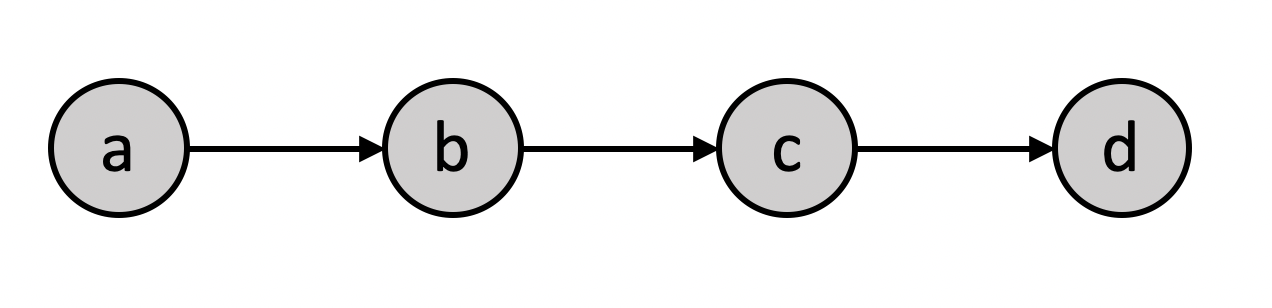
\includegraphics[width=2.5in]{prob3graph_forwards.png}
\end{figure}

Note that the order of vertices in this example is alphabetical in that $a < b < c < d$. Then, since we have defined this path of vertices to all be connected by forward edges, we will call \proc{Relax} on these edges in the order $(a,b), (b,c), (c,d)$ for some series of relaxations. Note that since there may exist other vertices and edges in this graph, this order is not strict. We are simply asserting $(a,b)$ will be relaxed before $(b,c)$, and so on. Therefore, if the shortest path estimate for vertex $a$ is correct (i.e. $a.d = \delta(s,a)$), then upon relaxing $(a,b)$, we will properly compute the shortest path estimate for vertex $b$. Then, when we relax $(b,c)$, we will properly compute the shortest path estimate for vertex $c$, and so on. The same can be said if each edge was a backward edge, not forward. In this case, such a path where $k=3$ would look like the following:

\begin{figure}[ht]
    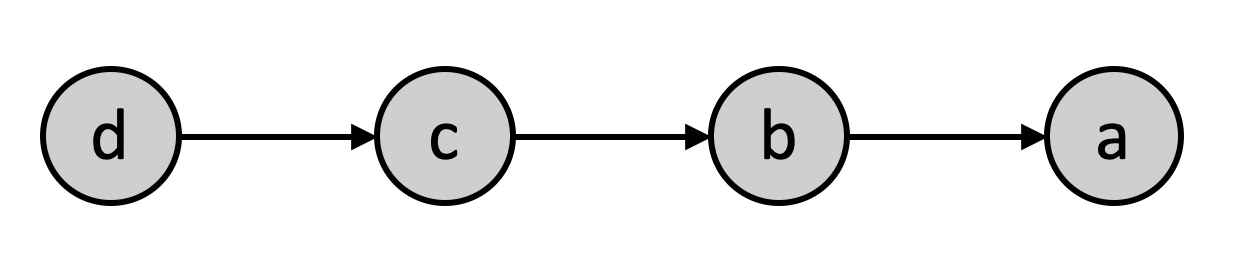
\includegraphics[width=2.5in]{prob3graph_backwards.png}
\end{figure}

Then, since we seek to estimate the shortest path from the source to each vertex, let us for the sake of this proof examine the worst-case scenario in which the shortest path $p$ from the source $s$ to vertex $v_{|V|}$ traverses each vertex $\{v_1, v_2, ..., v_{|V|}\}$ in some order. In this case, there exist $|V| - 1$ edges on the path $p$, some of which may be forward edges and some of which may be backward edges. In this case, we will correctly compute the shortest path weight for each vertex on a consecutive string of forward edges so long as the shortest path weight of the first vertex on the path is correct, and likewise for a consecutive string of backward edges. Then, we simply must prove it takes $|V| / 2$ sets of relaxations in order to properly set the shortest path estimate of the starting vertex on each set of consecutive direction edges.

To do so, let us note that the only case in which the shortest path estimate of the starting vertex of a set of consecutive direction edges will be incorrect is if there exists a change of direction on the path. Specifically, if $(v_{i-2}, v_{i-1}) \in E_f$ and $(v_{i-1}, v_i) \in E_d$, or vice versa. This is the case because we will no longer have a consecutive sequence of edges that we relax, and we therefore will relax other forward edges with incorrect values after relaxing $(v_{i-2}, v_{i-1})$ until we are able to come back on the second pass and set the value of $(v_{i-1}, v_i)$. Essentially, when there exists a change in direction, the first vertex in a series of consecutive direction edges beginning after a change in direction will be assigned an incorrect shortest path weight estimate, causing the shortest path weight estimate for each vertex on that series of consecutive direction edges to be incorrect.

Let us note, however, that since there exist $|V| - 1$ vertices on the path $p$ in question, there at most exist $|V| - 2$ changes in direction. Furthermore, on each series of relaxations, at least one shortest path estimate must be properly computed in $G$. Therefore, at least one incorrect shortest path estimate caused by a change in direction will be resolved on each pass of relaxations. Then, let us observe that on a single pass of relaxations, we iterate $2|V|$ times since each iteration of forwards and backwards edges (of which each edge is one or the other) will operate on each vertex twice, depending on if an edge leaves that vertex or not.

Therefore, we only need to pass over the edges $|V|/2$ times because we relax each edge exactly once on a given pass, we know there are at most $|V| - 2$ changes in direction, and we visit each vertex twice on a pass of relaxations. This indicates that we only need to pass over half the vertices in order to resolve each change in direction (i.e. properly set the shortest path estimate for the first vertex of a series of consecutive direction edges). Therefore, since we only need to visit half the vertices to resolve each change in direction (of which there are at most $|V| - 2$), we can iterate over the edges $|V| / 2$ times and we will have properly set the shortest path distance for each vertex. The logic behind this is that by relaxing edges in their consecutive direction order, once we properly set the shortest distance estimate of the first vertex on a string of consecutive direction edges, we will solve each vertex in a depth-first approach immediately after. Then, so long as we properly set the shortest distance estimate of the first vertex (which we have shown requires iterating over only one half of the vertices for a given pass of relaxations), we can efficiently solve the shortest path problem with just $|V|/2$ passes of relaxations and therefore just $|V|/2$ iterations over the edges.

Let us note that we require no negative weight cycles because we must guarantee we can set a solution for the starting vertex on each series of consecutive direction edges. With a negative weight cycle, each relaxation of a set of edges will decrease the shortest path estimate of some series of vertices, causing us to never converge on a proper solution. Essentially, the logic is the same as \proc{Bellman-Ford}.\\

\underline{\textbf{Part C:}} This run-time only decreases the coefficient in front of $VE$ from 1 to $\frac{1}{2}$. Therefore, we've only decreased the constant factor, indicating the asymptotic run-time has not changed since $O(1VE) = O(\frac{1}{2}VE) = O(VE)$.

\newpage

\section{Problem 4}
\separateline

\underline{\textbf{Part A:}} We can update the transitive closure $G^*$ in $O(V^2)$ time when a new edge is inserted into $E$ with the following. Let $(u,v)$ be the edge inserted into $E$. Then, since an edge existing in $G^*$ between any two vertices indicates there exists a path between them in $G$, upon inserting $(u,v)$ into $E$, we may have constructed a path between vertices that did not previously exist. This will require us to update the transitive closure by adding edges between now connected vertices in $G^*$. Let us note that a path will exist between two vertices $x,y$ in $G$ upon inserting $(u,v)$ into $E$ if there exists an edge $(x,u)$ in $G^*$ and an edge $(v,y)$ in $G^*$. In such a case, adding edge $(u,v)$ in $G$ constructed a path from $x$ to $y$ in $G$.

Therefore, we can update the transitive closure by iterating over all vertex pairs $x,y$ in $G$. For each, we can check if there exists a path from $x$ to $u$ in $G$ if there exists an edge $(x,u)$ in $G^*$. In order to determine if $(x,u)$ is in $G^*$, we simply must check if the value stored in the boolean matrix $c_{xu}$ is 1. The same process holds for checking if there is a path in $G$ from $v$ to $y$. Then, if both values are 1, we insert an edge $(u,v)$ in $G^*$ by setting $c_{uv} = 1$. The pseudocode for this algorithm is provided below.

\begin{codebox}
\Procname{$\procdec{Update-Transitive-Closure}(C, u, v)$}
\li \For $x \in V$ \Do
\li     \For $y \in V$ \Do
\li         \If $c_{xu} == 1 \land c_{vy} == 1$ \Do
\li             $c_{xy} = 1$
            \End
        \End
    \End
\end{codebox}\\

\\~

\underline{\textbf{Part B:}} Suppose we have the following graph $G$ and we just inserted the edge $(u,v)$ into $E$ (hence why it is dotted).

\begin{figure}[ht]
    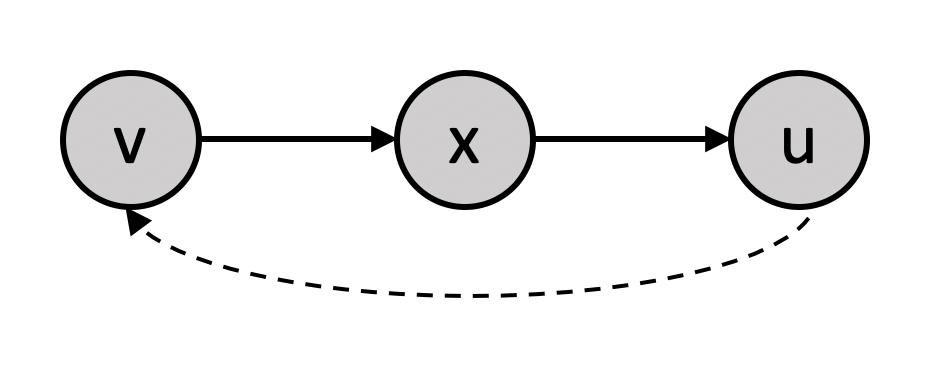
\includegraphics[width=2in]{prob4graph.png}
\end{figure}

Then, prior to inserting $(u,v)$ into $E$ our matrix $c$ is the following:


\begin{table}[H]
\begin{tabular}{l|llll}
  & $u$ & $v$ & $x$ &  \\
  \hline
$u$ & 1 & 0 & 0 &  \\
$v$ & 1 & 1 & 1 &  \\
$x$ & 1 & 0 & 1 &
\end{tabular}
\end{table}

Then, let us note that every edge in $G^*$ going from some other vertex to $u$ has a value of 1 and every edge in $G^*$ going from $v$ to some other vertex also has a value of 1. In this regard, there must exist an edge in $G^*$ for every possible combination of vertices since there now exists a path to and from all vertices in $G$. Therefore, regardless of what algorithm we use, we must make exactly $V^2 = 3^2 = 9$ updates to $G$. Therefore, we require $\Omega(V^2)$ time for updating the transitive closure in this case.\\

\underline{\textbf{Part C:}} First, let us note that since we have a directed graph, there can exist at most $(|V|)(|V|-1) = O(V^2)$ edges in the graph (since each vertex has an in-degree of at most $|V| - 1$). Therefore, for this problem let us consider the worst case scenario in which $m = O(V^2)$. This would occur when the graph begins with no edges, indicating the matrix $c$ holds entirely zeroes (except for the diagonal which is all 1 since you can get to and from the same vertex without an edge), then ends with a path between every possible vertex pair, indicating the matrix $c$ holds entirely ones.

Then, we seek to modify our updating mechanism to run in $O(V^3)$ time over all $O(V^2)$ insertions. In order to do this, let us observe that since we never remove edges from the graph $G$, once an edge exists in $G^*$ (i.e. a value in the $c$ matrix becomes 1), that edge will never be removed from $G^*$, so the value in the matrix will never again be 0. Therefore, if a value in the matrix is already 1, even if the conditions required to set it to 1 are satisfied, we are wasting computational resources by setting it to 1 again, since nothing about $c$ will have changed after doing so.

Then, let us think about the cases in which we know an edge must be inserted into $G^*$ (i.e. a value must be set from 0 to 1 in $c$). Intuitively, we only need to add edges to $G^*$ when the inserted edge connects two previously unconnected components. In such a case, the added edge bridges the two components together so certain elements in each are now reachable from each other. So, after the edge $(u,v)$ is inserted into $G$, we must add an edge to $G^*$ if and only if there exists a path $x \rightsquigarrow u$ in $G$ for some $x$ (indicating $u$ is reachable from $x$) and prior to inserting $(u,v)$, there did not exist a path $x \rightsquigarrow v$ in $G$. If this is the case, then we can get to $u$ from $x$ but we previously could not get to $v$ from $x$. This indicates that $x$ and $v$ were not connected before inserting $(u,v)$.

In such a case, since we know $(u,v)$ was added to $G$, we must now be able to reach $v$ from $x$ since $(u,v)$ bridges the connected components of $x$ and $v$. Then, since there exists a path from $x \rightsquigarrow u$ and an edge $(u,v)$ in $G$ and we know $c_{xv} = 0$ (since prior to $(u,v)$'s insertion, there did not exist a path from $x$ to $v$ in $G$), then we must have to insert $(x,v)$ into $G^*$, indicating we must have to set at least one value in $c$ to be 1. There may be more edges to insert because of this connection, but we know at least one must be inserted.

Using this, since there are at most $O(V^2)$ edges to be inserted into $G$, there are only $O(V^2)$ cases in which we know at least one edge must be inserted into $G^*$. For each of the $O(V^2)$ cases in which we know at least one edge must be inserted into $G^*$, we can then check for other possible edges to be added as well. Then, let us modify our algorithm from above to be the following:

\begin{codebox}
\Procname{$\procdec{Update-Transitive-Closure-Modified}(C, u, v)$}
\li \For $x \in V$ \Do
\li     \If $c_{xu} == 1 \land c_{xv} == 0$ \Do
\li         \For $y \in V$ \Do
\li             \If $c_{vy} == 1$ \Do
\li                 $c_{xy} = 1$
                \End
            \End
        \End
    \End
\end{codebox}

Essentially, this modification ensures that we only search for values to set to 1 in $c$ if we know at least one value in $c$ must be set to 1. This eliminates wasteful iterations when no changes must be made to $c$. In effect, we look at all vertices $x \in V$, and for each one, we search for other vertices with which to insert an edge into $G^*$ if we know we can get from $x$ to $u$ and we previously were unable to get from $x$ to $v$, but upon inserting $(u,v)$, we know we can now get from $x$ to $v$.

We can analyze the run-time of this algorithm as follows. The outer for-loop will iterate $O(V)$ times for each call to this function. The if-statement on line 2 will take constant time. This yields $O(V)$ for this section of the algorithm.

For the inner for-loop, let us observe that each time it runs, one value in $c$ must be 0 since the if-statement required to get to that section of the function requires $c_{xv} == 0$. Then, since we proved above that we must insert at least 1 edge into $G^*$ when this conditional holds, each time we iterate through the inner for-loop, we will set at least one value in $c$ from 0 to 1. Then, since the matrix $c$ holds $|V|^2$ values, the worst case scenario is when all $|V|^2$ values begin as 0. Then, as per the worst-case choice of $m$, we have $|V|^2$ values in $c$ to set to 1. Since at least one value in $c$ is set from 0 to 1 on a full-iteration of the inner-loop, the condition required to begin iterating through this loop will be satisfied at most $|V|^2$ times. Then, since the inner-loop iterates over all values in $V$, this inner loop will iterate a total of $O(V^2 * V) = O(V^3)$ times.

Therefore, the run-time of this algorithm across all $O(V^2)$ insertions is $O(V^2)*O(V) = O(V^3)$ for the outer for-loop and $O(V^3)$ for all runs of the inner for-loop, yielding a total run-time of $O(V^3)$.

\newpage

\section{Problem 5}
\separateline

For this problem, we seek to determine the minimum number of edges to remove from an undirected graph such that the graph becomes disconnected. Per CLRS 26.2, a flow network has a source vertex $s$ and a sink vertex $t$. We can construct a cut $(S,T)$ of a flow network $G=(V,E)$ that partitions $V$ into two sets $S$ and $T = V - S$ such that $s \in S$ and $t \in T$. The capacity of a cut $(S,T)$ is the sum of the capacities of each edge from a vertex in $S$ to a vertex in $T$, and a minimum cut of a network is a cut whose capacity is minimum over all cuts in the network.

Using these facts, let us observe the following. If the capacity of each edge in $G$ is 1, the minimum cut of a network with a pre-determined source and sink will be the minimum number of edges separating the source vertex (and perhaps some other vertices) from the sink vertex (and perhaps some other vertices) -- essentially, the minimum number of edges keeping the network connected. We know this to be the case because setting the capacity of each edge in $G$ to 1 acts as an indicator random variable. If an edge exists, its capacity is 1. If not, its capacity is 0. Then, the minimum number of edges separating a partition of the network is the minimum sum of the capacities of edges between all possible cuts of the network. In this regard, the minimum cut of a network is a possible number of edges required to disconnect the network.

Therefore, in order to determine the minimum number of edges to remove from an undirected graph such that it becomes disconnected, we simply must determine the minimum cut of the graph from some source vertex $s$. Let us observe, however, that the minimum cut of a graph changes depending on the chosen source vertex. This depends on how many outgoing edges the source vertex contains. Therefore, the minimum number of edges to remove from an undirected graph such that it becomes disconnected is the minimum cut of the graph for all possible source vertices.

In order to compute this minimum cut, we must convert our undirected graph $G=(V,E)$ into a flow network $G'$. To do so, we will first choose an arbitrary vertex $t \in V$ and denote that vertex as the sink. Then, we will iteratively perform the following for each source vertex $s \in V - \{t\}$. First, we will construct two directed edges in $G'$ for each undirected edge in $G$. Since a flow network cannot have anti-parallel edges, one of these directions will simply be between the two original vertices. For the other, we will construct a dummy vertex with two directed edges between them. For example, for the undirected edge $(u,v) \in G$, when creating the flow network $G'$, we will insert a directed edge from $u$ to $v$ in $G'$, then we will create a dummy vertex $x$ and insert a directed edge from $v$ to $x$ and a directed edge from $x$ to $u$ in $G'$. Performing this ensures that the number of edges crossing each cut is equal to the capacity of that cut. Then, we will set the capacity of each edge in the flow network to be 1. Let us note that this flow network then has $O(V+E)$ vertices because we have $O(V)$ vertices from $G$ and for each edge, we insert another vertex. Also note that this flow network has $O(E)$ edges because for each edge in $G$ there exist 3 edges in $G'$ and $O(3E) = O(E)$.

Then, we have constructed a flow network $G'$ that resembles our given undirected graph $G$. Then, we wish to compute the minimum cut of $G'$ for all possible source vertices. Note that the dummy vertices added when converting $G$ into the flow network $G'$ will not be considered possible source vertices since they do not exist in $G$. Then, in order to compute the minimum cut of $G'$ for each source vertex, let us simply compute the maximum flow of our flow network $G'$ by making a call to \proc{Edmonds-Karp}. By the Max-flow min-cut theorem (\textbf{Theorem 26.6}) in CLRS 26.2, the maximum flow $|f|$ of the flow network $G'$ is equal to the minimum cut $c(S,T)$ since the value of a maximum flow in a network is bounded above by the capacity of a minimum cut of the network. In fact, the value of a maximum flow is equal to the capacity of a minimum cut.

Then, our algorithm will be as follows. We will first set a variable $best$ to $\infty$ that will keep track of our best found minimum cut so far. We will then choose an arbitrary vertex $t \in V$ and denote that as our sink in $G'$. We will then construct our flow network as outlined above. Using this, for each vertex $s \in V - \{t\}$ (i.e. all those originally in $G$), we will compute the maximum flow (minimum cut) of $G'$ using $s$ as the source. If that value is smaller than $best$, we will update $best$. Then, after iterating over each possible source vertex, we will return $best$. Note that by the definition of a minimum cut, even though we added edges to $G'$, since each edge weight is 1, regardless of if the cut crosses the edge $(v,x)$ or $(x,u)$ following our example above, either one will indicate a capacity of 1 corresponding to the original undirected edge $(u,v)$ in $G$.

The run-time of our algorithm then is as follows. Since there exist $|E|$ edges in $G$ and we iterate over each when initially building the flow network, we have $O(E)$ pre-processing time for constructing the flow network and choosing the arbitrary sink vertex. Then, for each possible source vertex (of which there are at most $|V|$ since the added dummy vertices do not exist in $G$ and therefore cannot be source vertices), we make a call to \proc{Edmonds-Karp} in order to compute the maximum flow of a network with that source vertex. Since \proc{Edmonds-Karp} runs in $O(V^2E)$ time for a graph with $|V|$ vertices and $|E|$ edges, we then have $O((V+E)^2E)$ for each iteration since there exist $O(V+E)$ vertices and $O(E)$ edges in each flow network. This yields a final run-time of $O(VE(V+E)^2)$ for this algorithm.

\newpage

\section{Problem 6}
\separateline

In order to show that the subgraph-isomorphism problem is NP-hard, let us show that the clique problem can be reduced to the subgraph isomorphism problem in polynomial time. Note that a clique in an undirected graph $G = (V,E)$ is a subset $V' \subseteq V$ of vertices, each pair of which is connected by an edge in $E$, and that the clique problem is known to be NP-hard by \textbf{Theorem 34.11} in CLRS Chapter 34.5.

For the subgraph isomorphism problem at hand, we are given two undirected graphs $G_1$ and $G_2$, and must determine if $G_1$ is isomorphic to a subgraph of $G_2$. In other words, we must determine if there exists a subgraph $G'$ of $G_2$ with $|G_1.V|$ vertices such that we can relabel the vertices in $G_1$ to be vertices of $G'$ maintaining corresponding edges in each. Let us observe that a clique of any undirected graph by definition is fully connected. Therefore, if $G_1$ is fully connected and $G_1$ is isomorphic to a subgraph $G'$ of $G_2$, then $G'$ must be fully connected and it must contain a subset $V' \subseteq G_2.V$ of vertices, each pair of which is connected by an edge in $G_2.E$. Therefore, by the definition of a clique provided in CLRS Chapter 34.5, if $G_1$ is fully connected and $G_1$ is isomorphic to a subgraph $G'$ of $G_2$, then $G'$ must be a clique of size $|G_1.V|$ in $G_2$.

With this outline in place, we then must simply take an input to the clique problem and construct our $G_1$ and $G_2$ in polynomial time from it such that we have a valid input to the subgraph isomorphism problem. Since the clique problem receives as input a graph $G$ and an integer $k$, let us then perform the following. Let us construct a graph $G_1$ such that $G_1.V \subseteq G.V$, $|G_1.V| = k$, and $G_1$ is fully connected. In other words, let $G_1$ be some fully connected subgraph of $G$ that contains $k$ vertices. Then, let $G_2$ be $G$. Let us note that we can perform both transformations in polynomial time. Then, we can pass $G_1$ and $G_2$ to the subgraph isomorphism algorithm as outlined above. If there exists a clique of size $k$ in $G$, the subgraph isomorphism problem will return \textbf{True} since it will be able to construct the subgraph $G'$ from $G_2$ and will find that it is equal to $G_1$. If there does not exist a clique of size $k$ in $G$, then the subgraph isomorphism problem will return \textbf{False} since it will not be able to construct the subgraph $G'$ from $G_2$.

Therefore, we can take the input to the clique problem and shape it in polynomial time to an input to the subgraph isomorphism problem. Since the clique problem is NP-hard and we can formulate an input to it into an input to the subgraph isomorphism problem is polynomial time, then it must be the case that the subgraph isomorphism problem is NP-hard. Hence, the claim.

\newpage

\section{Problem 7}
\separateline

Let us note that a cyclic rotation between two strings $T_1$ and $T_2$ simply wraps the characters around such that the string $T_1$ can be found in a concatenation of $T_2$ with $T_2$. Following the example provided in the problem definition, $T_1$ = "braze" and $T_2$ = "zebra" are cyclic rotations of each other with $r = 2$ because "braze" exists in "ze\textbf{braze}bra." That is, "braze" exists in a concatenation of "zebra" + "zebra."

Therefore, given two length $m$ strings, we can determine if they are cyclic rotations of each other using $\Theta(m)$ pre-processing time and $\Theta(m)$ matching time
by simply calling \proc{Knuth-Morris-Pratt} on $T_1$ and $T_2T_2$. Since we are looking for a length $m$ pattern in a length $2m$ string, this yields a pre-processing time of $\Theta(m)$ and a matching time of $\Theta(2m) = \Theta(m)$.

\newpage

\section{Problem 8}
\separateline

In order to prove this heuristic returns a tour whose total cost is not more than twice the cost of an optimal tour for the traveling-salesperson problem, let us observe that the method outlined in the problem definition is a description of \proc{MST-Prim} for computing a minimum spanning tree of an undirected weighted graph $G$, but uses a cycle rather than a tree.

\proc{MST-Prim} begins by taking a source vertex and setting the shortest path estimate $v.d$ for all vertices $v \in V$ to $\infty$. It then sets the shortest path estimate for the root to be 0. It then constructs a priority queue and inserts each vertex in the graph to the queue. Then, \proc{MST-Prim} iteratively pulls vertices out of the priority queue in order of their shortest path estimate. In this regard, any vertex that is in the queue is not in the minimum spanning tree and the vertex returned by \proc{Extract-Min} is the vertex with the smallest shortest path estimate in the graph. When a vertex $u$ is extracted, we then iterate through all vertices $v$ in $u$'s adjacency list. If the shortest path estimate of $u$ plus the weight of the edge $(u,v)$ is less than the shortest path estimate of $v$, we then update the shortest path estimate of $v$ since we have found a more optimal path by setting $v.d = u.d + w(u,v)$ then setting $v.\pi = u$. In this regard, the vertex returned by \proc{Extract-Min} is the vertex that is not in the tree, but whose distance to any vertex in the tree is minimum. By extracting this vertex from the queue, we insert it into the tree.

Then, we can formulate this process into a cycle rather than a minimum spanning tree by observing that the pre-order walk of a minimum spanning tree $T$ from the root forms a cycle. This is the case because any pre-order walk of a tree will visit each non-leaf vertex at least twice. Immediately upon coming across a vertex, the pre-order walk visits that vertex, then visits all children to the left, then comes back to the vertex, then visits all children to the right, and returns. Then, since the walk starts at the root, it will explore all children to the left, then to the right, then will return to the root.

Therefore, when iteratively building a minimum spanning tree from a root vertex in \proc{MST-Prim}, we are also building a cycle since any pre-order walk of a tree forms a cycle. Therefore, the order of the vertices added to the tree in \proc{MST-Prim} is identical to the order of the vertices added to the cycle in this heuristic. In this regard, even though we never build a minimum spanning tree in this algorithm, the processes and order of vertices added are identical in both algorithms.

Then, we can reformulate this closest-point heuristic by considering the case in which we construct a minimum spanning tree $T$ from an arbitrary root vertex $r$ in $G$ by calling \proc{MST-Prim}, then perform a pre-order walk of $T$ from the root and construct a list of visited vertices. Since we showed above that the pre-order walk may visit a vertex more than once, we will construct this list such that it is ordered according to when a vertex is first visited in the pre-order walk of the tree. Let us refer to this list as $H$. Then, since it was shown above that the order of vertices added to the cycle in the given algorithm is identical to the order of vertices added to the minimum spanning tree in this reformulated solution, all we must do is return $H$ since $H$ will be identical to the output from the given algorithm. Let us observe that this reformulated solution is identical to \proc{Approx-TSP-Tour} from CLRS 35.2.1

Then, since we can compute \proc{MST-Prim} and can perform a pre-order walk of any tree in polynomial time, we have that this heuristic will run in polynomial time. Then, all that we must prove is that the result returned from this algorithm outlined above is a tour that has a cost no more than twice the cost of an optimal tour. Since we showed that the output from the reformulated solution is identical to the output from the given algorithm, and we showed that the reformulated solution is identical to \proc{Approx-TSP-Tour} from CLRS 35.2.1, by \textbf{Theorem 35.2}, we have that \proc{Approx-TSP-Tour} is a polynomial-time 2-approximation algorithm for the traveling-salesperson problem with the triangle inequality. Therefore, this heuristic returns a tour whose total cost is not more than twice the cost of an optimal tour, assuming the triangle inequality holds, since the outputs and processes of each algorithm are the same.

\newpage

\end{document}
